\part{Special Relativity}
\chapter{Introduction}
\section{The problem of abstract definitions}
Let's start our discussion about Special Relativity by redefining some fundamental quantities. Since the beginning of science defining basic principles was challenging, even some great scientists of the past tried to give definitions of fundamental concepts. For example:
\begin{quotation}
  \noindent\textit{I do not define time, space, place, and motion, as being well known to all. Only I must observe that the common people conceive those quantities under no other notions but from the relation they bear to sensible objects. And thence arise certain prejudices, for the removing of which it will be convenient to distinguish them into absolute and relative, true and apparent, mathematical and common.}
  \begin{enumerate}
    \item \textit{Absolute, true, and mathematical time, of it self and from its own nature, flows equably without relation to anything external, and by another name is called 'duration'; relative, apparent, and common time is some sensible and external (whether accurate or unequable) measure of duration by means of motion, which is commonly used instead of true time, such as an hour, a day, a month, a year.}
    \item \textit{Absolute space, in its own nature, without relation to anything external, remains alwayas similar and immovable. Relative space is some movable dimension or measure of the absolute spaces, which our senses determine by its position to bodies and which is commonly taken for immovable space; such is the dimenion of a subterraneous, an aerial, or celestial space, determined by its position in respect of the earth.}
  \end{enumerate}
  \noindent\rule{\linewidth}{0.4pt}

  \hfill Sir Isaac Newton, \textit{Principia Mathematica}
\end{quotation}
This is a typical abstract definition. In a mathematical approach it does not matter if the definition doesn't match something really existent in our world, since it is used as a mathematical base to derive other concepts. Another example would be the definition of ``straight line'', there is no such thing in reality, but its definition is useful in a mathematical context.\\
This is where Einstein's revolutionary view starts. Einstein stated that Newtonian mechanics was false due to its relying on \textbf{metaphysical} concepts rather than facts coming from the experience. Given this he also gave a completely new point of view of the definitions of the fundamental quantities of mechanics, with a physical/\textbf{empirical} approach. All of Einstein's relativity naturally stems from the definitions given at the start.\\
But now we should ask ourselves: ``How do we define quantities in an empirical way?''\\
To answer this we should look at how we can experience the world. We interact with physical objects by doing \textbf{measurements}, and so we must state our definitions in an \textbf{operational} way.\\
There are two main advantages of this way of thinking:
\begin{enumerate}
  \item Since we are basing our definitions on measurements there is no risk for our definitions to diverge from our understanding of the world
  \item If our technological capabilities or theories evolve to get more accurate results we should simply extend our definitions in order to match the new data
\end{enumerate}
In principle avoiding abstract definitions will prevent the need of new conceptual revolutions to correct previous mistakes, caused by the misinterpretation of concepts. Instead, every update of our understanding of the world should naturally come from the extension of our definitions.\\
For example if we define length as ``the quantity measured by a rigid ruler'' we can obviously use this definition only for local applications, but for astronomical distances this definition is not applicable, thus we need to define a new way of measuring length, but the two definitions must coincide where they can both be applied.
\section{Basic concepts}
Finally, after establishing a new way to define quantities, we can start giving definitions of some basic concepts.
\begin{definition}{Event}
  An event is a phenomenon that occurs in a region of space so small that it can be considered a point, and in a time interval so short that it can be considered an instant.
\end{definition}
The event is the simplest element of a physical description. Let's notice that to give the description of an event we used not only space coordinates, but we also introduced time as a fourth coordinate.\\
From the definition of event we can start to describe more general phenomena. For example if something is occuring for a continuous duration in time ``the pen is at rest on the desk'', in principle we should describe this as a series of events with the same space coordinates, but with evolving time coordinate. Instead, if something happens at the same moment in time, but in two different places we should describe this as two events with the same time coordinate, but different space coordinates.\\
In order to talk about coordinates we need a new tool:
\begin{definition}{Reference frame}
  A reference frame is a physical system, or a set of systems, that allows labelling the events with space and time coordinates.
\end{definition}
But how do we label events in space? We should define a metric, and so a length, in physical space to measure distance between objects, but first we need to define physical space:
\begin{definition}{Physical space}
  We will call ``physical space'' the set of all possible relative positions of rigid bodies.
\end{definition}
From this definition it is reasonable to define length as something measured by the means of a rigid body, chosen arbitrarily and conventionally to be of length 1. To define length in an operational way we must explicitly define every step in order to measure is:
\begin{definition}{Operational definition of length}
  \begin{enumerate}
    \item Define what length is: ``Length is the quantity that can be measured with a ruler''
    \item Define an empirical ruler (i.e. a bar of metal)
    \item Define what we mean when we say that ``two objects have the same length''. This also allows us to say that, for any pair of points $A$ and $B$, their distance coincides with the distance between the point $A'$ and $B'$ on the ruler that correspond to $A$ and $B$ \label{d:lengthp3}
    \item Define what we mean when we say that ``the length of the object $C_3$ is the sum of the lengths of the objects $C_1$ and $C_2$''. This allows defining multiples and sub-multiples \label{d:lengthp4}
    \item Define a unit. In the SI the unit is the metre, that has long been, by definition, the length of a Pt-Ir bar kept in the Laboratoire des Poids et des Mésures in Sèvres, France.
  \end{enumerate}
\end{definition}
From this definition we know that the rigid ruler must be \textbf{invariant under translations} in space, since by point \eqref{d:lengthp3} and \eqref{d:lengthp4} we need to be able to tell if two objects have the same length (congruence), and we need to be able to move our ruler (translation). Also, we must impose that the ruler is \textbf{straight} in order to measure the minimum distance between objects. But what means straight? As we said earlier there is no straight line in reality, but the best approximation is:
\begin{definition}{Straight line}
  A light beam that travels in a vacuum
\end{definition}
This definition is also useful to measure astronomical distances since the only way we have to get information about distant planets is through the light beams that come from space. This definition must also be consistent with the definition of the rigid ruler, thus the rigid ruler must be parallel to a light beam that travels in a vacuum.\\
This property has also led to the current definition of the metre in the SI units:
\begin{definition}{Metre}
  The metre, symbol m, is the SI unit of length. It is defined by taking the fixed numerical value of the speed of light in a vacuum, $c$, to be $299792458$ when expressed in $\unit{\metre \second^{-1}}$.
\end{definition}
All considered, our final definition of a rigid ruler is:
\begin{definition}{Rigid ruler}
  A rigid ruler is an empirical ruler such that:
  \begin{enumerate}
    \item is invariant under translations in space
    \item is straight with respect to the light beams propagating in vacuum
    \item is graduated in metres and their sub-multiples.
  \end{enumerate}
\end{definition}
Now we can introduce some final key elements. The first one is the interial frame of reference \textbf{IRF}:
\begin{definition}{Interial reference frame (I)}
  A reference frame is said to be interial if:
  \begin{enumerate}
    \item the space is Euclidean (and in particular is homogeneous and isotropic) with respect to our definition of length
    \item a free particle intially at rest remains indefinitely at rest.
  \end{enumerate}
\end{definition}
Does this definition make sense? For this definition to be useful we must admit that there exists at least one IRF (for example the centre of mass of the Universe) and verify this \textit{a posteriori}.\\
Finally, we should define the concept of time, but defining time in an operational way is hard since there cannot be a direct comparison with a homogeneous quantity for time measurements. For this reason we first need to define an instrument capable of measuring time. Since the origin of humanity time has been essentially measured by counting the repetitions of a periodic motion. First we had moon cycles, then the movement of a mechanical gear and finally, with modern technology, we measure the oscillations of materials or atoms (quartz clocks and atomic clocks). Given this we can define the clock as:
\begin{definition}{Clock}
  A clock is a physical system that counts the oscillations of a periodic motion.
\end{definition}
By this definition we assume that:
\begin{enumerate}
  \item We need to choose a ``fundamental periodic motion'' that we assume to be isochronic by convention
  \item The fundamental periodic motion can be used as a ``metronome'' and we will call clock any system which
  is able to count the number of its oscillations
\end{enumerate}
From this we can define the unit of time as the time interval required for a certain number of such oscillations::
\begin{definition}{Second}
  The second is the duration of 9192631770 periods of the radiation corresponding to the transition between two hyperfine levels of the ground state of the caesium-133 atom.
\end{definition}
Any other motion will be described in terms of the fundamental periodic motion. For example a generic uniform periodic motion such that:
\begin{equation}
  \theta = \omega t
\end{equation}
Is described as:
\begin{equation}
  \theta = \omega n T
\end{equation}
Where $T$ is the fundamental period and $n$ is the number of fundamental periods in a second.\\
Now we can use the second part of Newton's First law in order to choose the fundamental periodic motion:
We will have to choose the fundamental isochronic motion such that, in an IRF a free particle moves along a straight line covering equal distances in equal intervals of time. The clock with respect to which this is true is called \textbf{inertial clock} and the time it measures is called \textbf{inertial time}:
\begin{definition}{Inertial clock}
  A clock is said to be intertial if, in an inertial reference frame, the time intervals required for a free particle to cover equal distances are found to be equal, if measured with that clock.
\end{definition}
This definition means that inertial clocks are local and so an inertial clock can only measure the time in the point where it is placed in space. We cannot measure a series of events that are not happening in the point we placed the clock. If we want to do so, we need to put another clock in the other point that is synchronized with the original clock. The process of synchronization is not trivial and will be discussed later.\\
Finally, considering the notions we gave for time and clocks we will give a new definition for the inertial reference frame:
\begin{definition}{Inertial reference frame (II)}
  A reference frame is inertial if it is equipped with rigid rulers and clocks with respect to which:
  \begin{enumerate}
    \item the space is Euclidean
    \item the principle of inertial holds, i.e.: a free particle at rest remains indefinitely at rest, and a free particle in motion travels equal distances in equal times along a straight line.
  \end{enumerate}
\end{definition}
This definition has a huge consequence, in fact, given the fact that there exists at least one IRF, then there is an infinite number of IRF as well.
\section{Galilean transformations}
Galilean transformations generate from the fact that Newton's laws are invariant under the change of a IRF. This means that there is no experiment in mechanics that would imply the existence of a privileged reference frame, thus we cannot distinguish a concept of absolute motion or absolute rest. Let's take:
\begin{itemize}
  \item $\irf{R}$ and $\irf{R'}$ are both IRFs
  \item $\irf{R'}$ is in motion with respect to $\irf{R}$ with constant velocity $\vec{v}$
  \item Rotate the axes until $\vec{v} \parallel x$ and $\vec{v} \parallel x'$
  \item Rotate the axes until $x \parallel x'$, $y \parallel y'$ and $z \parallel z'$, in particular the axes $x$ and $x'$ are coincident
\end{itemize}
An event can either be expressed in terms of $\irf{R}$ coordinates $(x,y,z,t)$ or $\irf{R'}$ coordinates $(x',y',z',t')$, actually, in a Galilean transformation $t=t'$.\\
The two systems are said to be in \textbf{standard configuration} if $O=O'$ at time $t=t'=0$. In a generic time $t\neq 0$ the transformation of the coordinates is:
\begin{equation}
  \begin{cases}
    x = x' + vt\\[8pt]
    y = y'\\[8pt]
    z = z'\\[8pt]
    t = t'
  \end{cases} \longrightarrow \quad
  \begin{cases}
    x' = x - vt\\[8pt]
    y' = y\\[8pt]
    z' = z\\[8pt]
    t' = t
  \end{cases}
\end{equation}
We can easily see this since the $y$ and $z$ coordinates do not change over time by consturction, instead the $x$ and $x'$ coordinates move with respect to one another with velocity $v$. Let's also notice that the geometrical distance of points is invariant:
\begin{equation}
  \begin{split}
    d(P_1,P_2) &= \sqrt{(x_1 - x_2)^2 + (y_1 - y_2)^2 + (z_1 - z_2)^2} =\\[8pt]
    &= \sqrt{(x'_1 + \cancel{vt} - x'_2 - \cancel{vt})^2 + (y'_1 - y'_2)^2 + (z'_1  - z'_2)^2} =\\[8pt]
    &= \sqrt{(x'_1 - x'_2)^2 + (y'_1 - y'_2)^2 + (z'_1  - z'_2)^2} = d(P'_1,P'_2)
  \end{split}
\end{equation}
Going back to the transformation equations we can differentiate them with respect to time and obtain that:
\begin{equation}
  \begin{cases}
    x' = x - vt\\[8pt]
    y' = y\\[8pt]
    z' = z
  \end{cases}
  \overset{\frac{\dd{}}{\dd{t}}}{\longrightarrow} \quad
  \begin{cases}
    u_x' = u_x - v\\[8pt]
    u_y' = u_y\\[8pt]
    u_z' = u_z
  \end{cases}
\end{equation}
If we further differentiate with respect to time:
\begin{equation}
  \begin{cases}
    u_x' = u_x - v\\[8pt]
    u_y' = u_y\\[8pt]
    u_z' = u_z
  \end{cases}
  \overset{\frac{\dd{}}{\dd{t}}}{\longrightarrow} \quad
  \begin{cases}
    a_x' = a_x\\[8pt]
    a_y' = a_y\\[8pt]
    a_z' = a_z
  \end{cases}
\end{equation}
Thus $\vec{a}' = \vec{a}$, and so writing Newton's second law in the two IRFs will give:
\begin{equation}
  \begin{split}
      &\bigsum \vec{F} = m \vec{a} \quad \quad \quad \quad \quad \text{in } \irf{R}\\[8pt]
      &\bigsum \vec{F} = m \vec{a}' = m \vec{a} \quad \quad \text{in } \irf{R'}
  \end{split}
\end{equation}
This means that Newton's second law is invariant under galilean transformations, which also implies that all classical mechanics is invariant under galilean transformations. As mentioned before we can state the principle of galilean relativity:
\begin{theorem}{Galilean relativity}
  No experiment of mechanics in an IRF can tell anything about the motion of this IRF with respect to other IRFs
\end{theorem}
\section{The problem of galilean relativity}
\subsection{Electromagnetism does not respect galilean relativity}
Now the real problem arises, in fact Electromagnetism \underline{is not invariant} under galilean transformations. Let's see the effect of galilean transformation on Lorentz force, in an IRF:
\begin{equation}
  \vec{F} = q\brackets{\vec{E} + \vec{u} \cross \vec{B}}
\end{equation}
If Electromagnetism was invariant under galilean transformations then:
\begin{equation}
  \vec{F}' = q\brackets{\vec{E}' + \vec{u}' \cross \vec{B}'} \overset{!}{=} \vec{F}
\end{equation}
To verify this we simply extend the equations:
\begin{equation}
  \begin{split}
    q\vec{E}' + q\brackets{\vec{u}-\vec{v}} \cross \vec{B}' &= q\vec{E} + q\vec{u}\cross \vec{B} \\[8pt]
    \vec{E}' + \vec{u} \cross \brackets{\vec{B}'-\vec{B}}  &= \vec{E} + \vec{v}\cross \vec{B}'
  \end{split}
\end{equation}
For this to be true we need:
\begin{equation} \label{e:false_conditions}
  \begin{split}
    &\vec{B}' = \vec{B}\\[8pt]
    &\vec{E}' = \vec{E} + \vec{v} \cross \vec{B}' = \vec{E} + \vec{v} \cross \vec{B}
  \end{split}
\end{equation}
But if we put our new fields back into \maxwellref\;we can see that those cannot be solutions.\\
Let's make another example. In our first frame of reference $\irf{R}$ we take a positively charged cable along the $x$ axis and a point $P$ stationary with respect to the cable.
\begin{figure}[H]
  \centering
  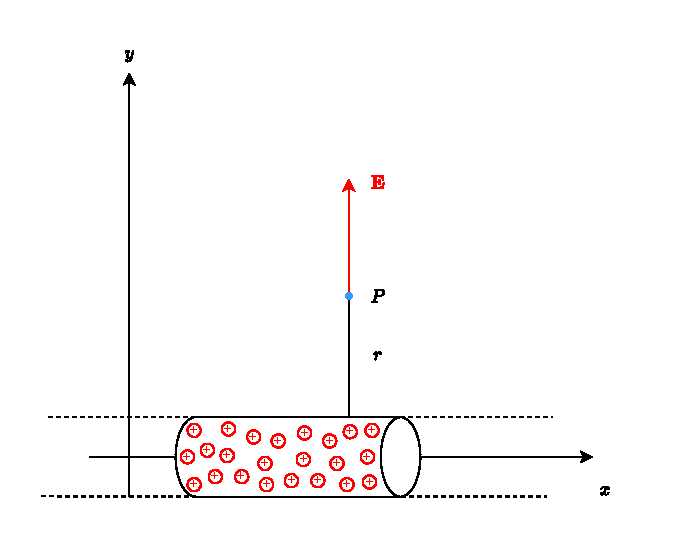
\includegraphics[width=0.6\linewidth]{res/svg/stationary_cable.drawio}
  \caption{Frame of reference $\irf{R}$}
\end{figure}
The point is at distance $r$, in the $y$ axis, from the cable, thus in $P$ there will be an electric field:
\begin{equation}
  \vec{E} = \dfrac{1}{2 \pi \epsz}\dfrac{\lambda}{r}\hat{u}_y
\end{equation}
Since the second IRF $\irf{R'}$ will in general be moving with respect to $\irf{R}$ with $\vec{v} \neq 0$, the point $P'$ will see charges in motion in the new frame of reference.
\begin{figure}[H]
  \centering
  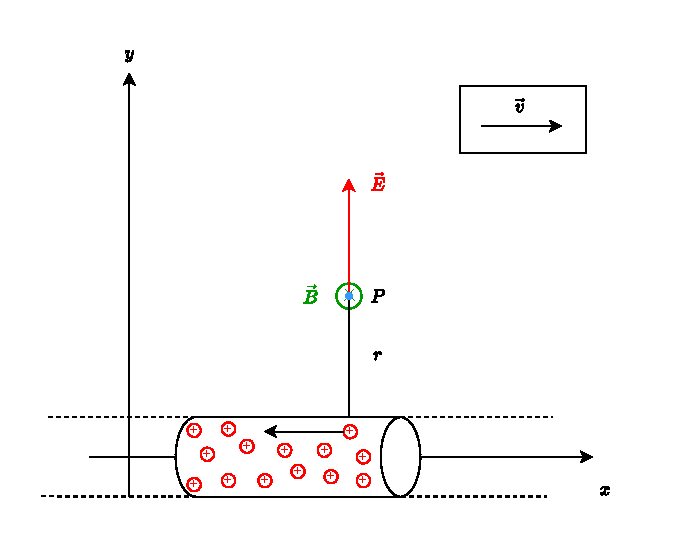
\includegraphics[width=0.6\linewidth]{res/svg/moving_cable.drawio}
  \caption{Frame of reference $\irf{R'}$}
\end{figure}
The linear charge density will be the same, since if one charge enters the ``field of view'' of $P$ another exits it, but, in this case $P'$ will also feel a magnetic field:
\begin{equation}
  \vec{B}' = \dfrac{\muz}{4 \pi}\dfrac{i}{r}\brackets{-\hat{u}_z}
\end{equation}
But, by actually measuring the fields in that point in space we do not see the effect of this seamingly ``newly-generated'' magnetic field. Also, if we check the conditions we got in \eqref{e:false_conditions} we can immediatly see that they are not satisfied.\\
Another example of the non-invariance of Electromagnetism are the potential equations in a vacuum at long distances:
\begin{equation}
  \begin{split}
    &\dalop \potE = 0\\[8pt]
    &\dalop \vec{A} = 0
  \end{split}
\end{equation}
The D'Alembert operator is not invariant under galilean transformations, in fact it would result that:
\begin{equation}
  \dalop = \dalop' -\dfrac{v^2}{c^2} \dfrac{\partial^2}{\partial x'^2} + \dfrac{v^2}{c^2} \pdv{}{x'}{t'}
\end{equation}
After those examples, if we want to preserve galilean transformations we must assume that there is only one IRF in which \maxwellref\;are true.\\
In order to try to solve this problem a new medium for electromagnetic waves propagation was hypotized and was called the \textbf{ether}, or, in latin \textit{etere luminifero}.\\
This new medium was defined more in a mathematical way rather than a physical one (and as we disucssed this is an issue). In fact, it was defined through the property it must satisfy.
Ether must:
\begin{itemize}
  \item be completely transparent to electromagnetic radiation
  \item have zero viscosity
  \item permeate all space
\end{itemize}
With the introduction of this new medium scientists supposed that \maxwellref\;may be true only in the IRF in which the motion of ether is stationary, so let's call:
\begin{quote}
  $\mathbfcal{R}_0$ is the only IRF (in which the ether is at rest) where the laws of Electromagnetism are true.
\end{quote}
This way of reasoning was not so new as we might think, since this would be the case for classical mechanical waves. If the medium of a wave goes faster/slower, then the wave itself goes faster/slower, we can only observe the ``pure'' wave motion if we are stationary with respect to the medium the wave is propagating inside.\\
Actually there was also another problem, since light travels at constant velocity $c$ in every direction we could find the only IRF in which this is true, but this is actually $\mathcal{R}_0$. This contradicts galilean relativity and would mean that electromagnetic measurements could tell us how any other IRF is moving with respect to $\mathcal{R}_0$. For this reason we can also define $\mathcal{R}_0$ as:
\begin{quote}
  $\mathbfcal{R}_0$ is the only optically isotropic reference frame
\end{quote}
\subsection{Michelson-Morley experiment}
There is a well-known experiment which wanted to prove the existence of ether, this experiment is known as the \textbf{Michelson-Morley experiment}. The two scientists created a setup consisting of an interferometre, a device in which a laser beam, generated by a source, splits into two other beams which travel along identical arms and then get reflected back into a screen.\\
The experimental setup is:
\begin{figure}[H]
  \centering
  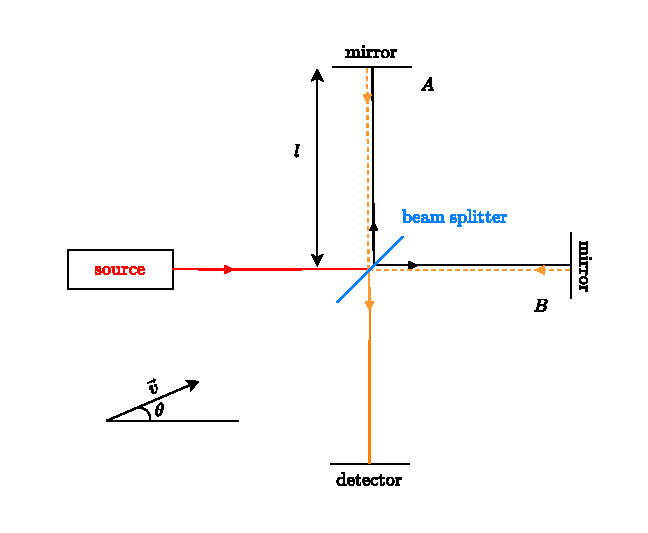
\includegraphics[width=0.6\linewidth]{res/svg/michelson_morley_experiment.drawio}
  \caption{Michelson-Morley interferometre}
\end{figure}
Since, at least once a year, Earth is moving with respect to the ether the two beams should take different paths with different length. This would mean that we should see an interference pattern appearing on the screen which will depend on the difference in time it takes to travel part A and part B. By doing the calculations we get:
\begin{equation}
  \Delta t = t_A - t_B = \dfrac{l}{c}\brackets{\dfrac{v}{c}}^2\cos(2\theta)
\end{equation}
So by moving the experimental setup, and thus changing the value of $\theta$, we might expect to see a difference in the measured time difference, but this was not the case. The measurements were conducted in different times of the year, but the results were pretty much against the hypotesis of ether. There were two possible explainations:
\begin{enumerate}
  \item Earth \underline{is} $\mathcal{R}_0$ and so light travels in any direction with speed $c$
  \item The ether has some sort of ``drag effect'' which would affect the experimental results
\end{enumerate}
The first explaination is just really unlikely, the second one contradicts the definition of ether itself, we would need an ether that both has zero viscosity, but also generates a drag effect. This basically makes zero sense.
\subsection{Stellar aberration}
Another contradiction of the ether model arises from the observation of a phenomenon called \textbf{stellar aberration}. Let's imagine that we want to capture the light emitted by a far away star. In order to do this we must put our telescope at an angle $\alpha$ since Earth is moving with respect to ether.
\begin{figure}[H]
  \centering
  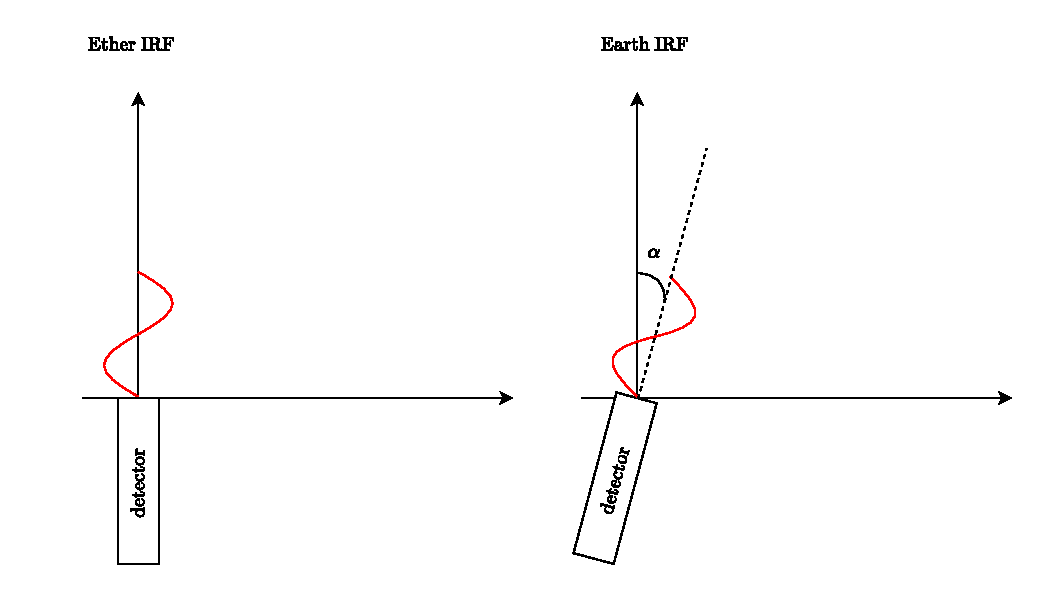
\includegraphics[width=0.6\linewidth]{res/svg/stellar_aberration.drawio}
  \caption{Stellar aberration}
\end{figure}
In particular, the angle must be the angle for which this condition is true:
\begin{equation}
  \tan \alpha = \dfrac{v}{c}
\end{equation}
Where $v$ is the velocity of Earth with respect to ether. According to the data collected by measurements $v \approx 3100 \unit{\meter / \second}$. This means that Earth should be moving with respect ot ether and this already contradicts the hypotesis that requires the IRF to be the same as the ether one. And so the explaination which considers the existence of ether for the Michelson-Morley experiment is not compatible with experimental data, therefore it must be rejected.
\subsection{Emission theory}
After the previous theories were rejected a new model was created. This is the \textbf{emission theory} model, which is based on some key concepts:
\begin{itemize}
  \item There is no ether
  \item There is no optically isotropic IRF
  \item Every source emits electromagnetic waves isotropically in their reference frame, which means that every IRF is isotropical for its radiation
\end{itemize}
This explains both the phenomenon of stellar aberration since the IRF of Earth is not the same as the source of the light, and it also explains Michelson-Morley experiment. Unfortunately this is not the case. To prove this we will now introduce an experimental observation that contradicts this theory.
\subsection{Binary stars}
Let's consider a system of two stars orbiting around each other. This system was described in 1913 by  Willem de Sitter.
\begin{figure}[H]
  \centering
  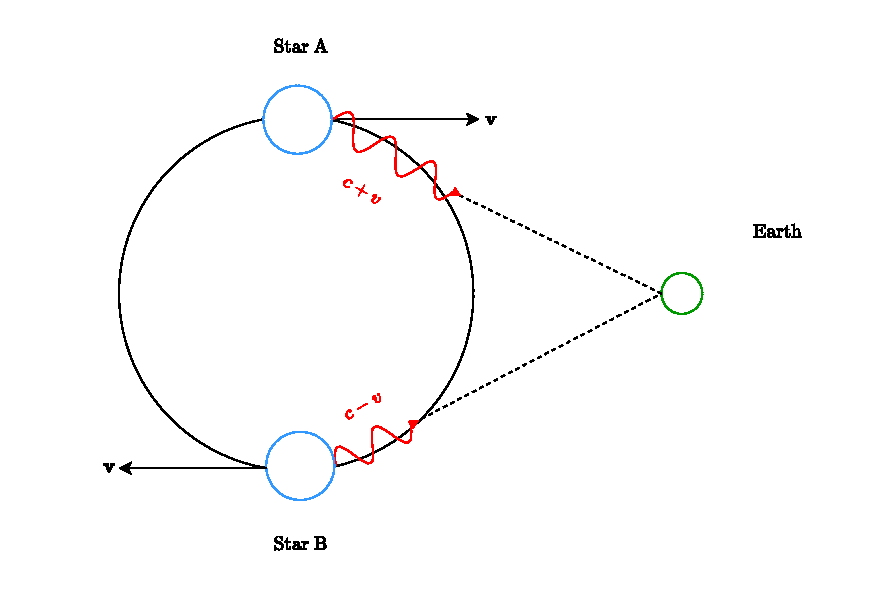
\includegraphics[width=0.6\linewidth]{res/svg/binary_stars.drawio}
  \caption{Binary stars system}
\end{figure}
If we apply the emission theory model we should expect to see that the intensity of light reaching us has some sort of periodic non-constant pattern, instead, experimental observation lead to seamingly unexplainable data. The intensity of the radiation was constant for most of the time and a minimum was periodically registered. The minimum of intensity corresponds with an eclipse event or, in other terms, when one of the stars covered the other and blocked its light.\\
One last attempt to save the ether hypotesis was done by introducing a correcting factor:
\begin{equation}
  \gamma = \dfrac{1}{\sqrt{1-\dfrac{v^2}{c^2}}}
\end{equation}
This factor was present in a new given hypotesis:
\begin{itemize}
  \item Lengths contract with a factor of $\gamma$ if the body is in motion with respect to Ether
  \item Clocks slow down with a factor of $\gamma$ if the body is in motion with respect to Ether
\end{itemize}
This factor was called \textbf{Lorentz factor} in the name of Hendrick Lorentz. The hypotesis of length contraction and time dilation was, at that time, just an \textit{ad hoc} hypotesis and was later proved to be insufficient to explain a Michelson-Morley type of experiment with different arms length. But as we might notice this already starts to look like something very similar to Einstein's hypotesis for Special Relativity, in fact the Lorentz factor was later used to develop \textbf{Lorentz transformations}, which are the starting point of Special Relativity.
